\chapter{The FPGA}
\label{cha:fpga}

\section{Opal Kelly}
\label{sec:fpga-opal}
The design is based on the XEM7310-A75 board. This is a USB 3.0 FPGA development board, featuring the Xilinx Artix-7 FPGA. The board is designed to boost productivity and testing capabilities of digital designs, providing ease of communication with its USB host interface. A Block Diagram of the device is provided in figure \ref{fig:xem-block-diagram}.
\begin{figure}
    \centering
    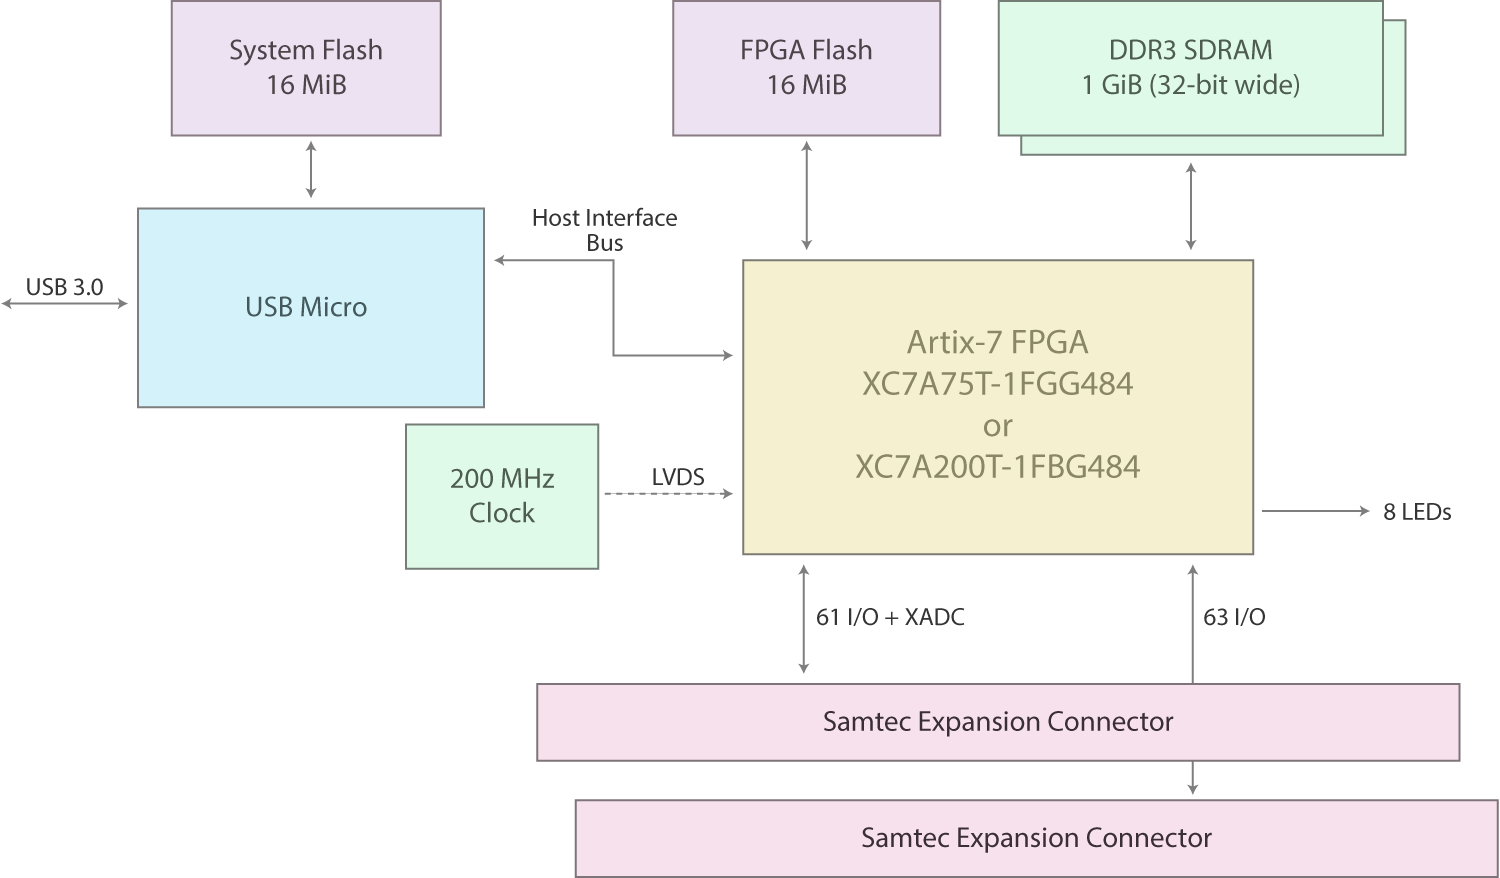
\includegraphics[width=0.5\linewidth]{lt_bachelor_disi_en//images/2XEM7310-BlockDiagram.png}
    \caption{XEM7310-A75 Block Diagram}
    \label{fig:xem-block-diagram}
\end{figure}

In particular, Opal Kelly provides an SDK (Software Development Kit) composed of several HDL modules, for example:
\begin{itemize}
    \item Virtual Trigger signals
    \item Two Pipes (in / out) for fast communication between FPGA and a host pc
    \item Much more
\end{itemize}
This is a sketched overview:
\begin{figure}
    \centering
    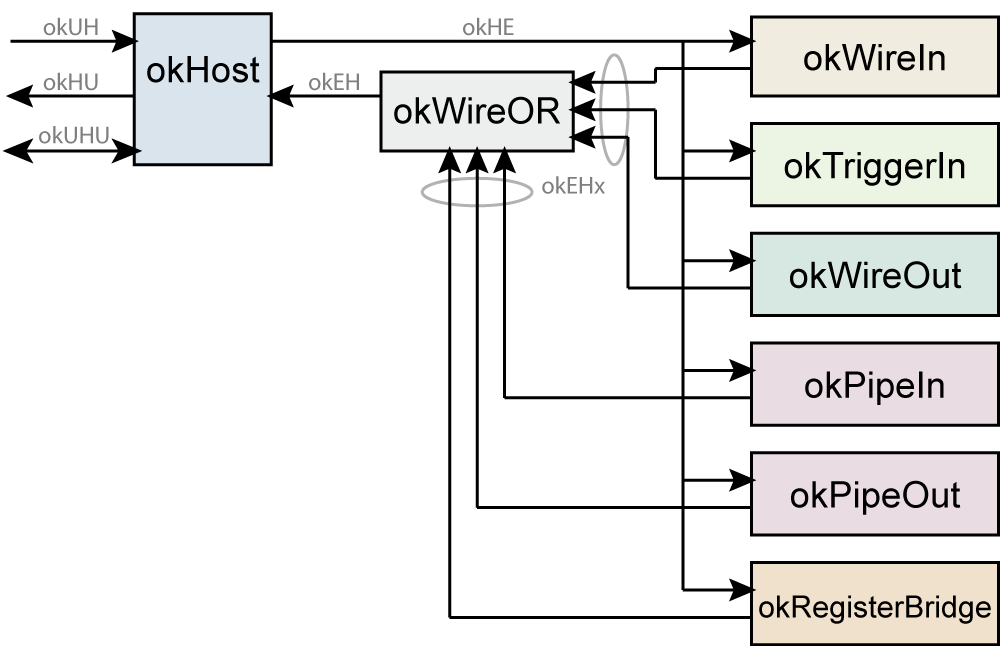
\includegraphics[width=0.5\linewidth]{lt_bachelor_disi_en//images/FrontPanelHDL-USB3.png}
    \caption{Opal Kelly HDL Overview}
    \label{fig:opal-kelly-hdl}
\end{figure}


\section{Xilinx Artix 7}
\label{sec:fpga-artix}
The specific FPGA mounted on the XEM7310-A75 is a Xilinx Artix-7. In particular, the model is the XC7A75T-1FGG, featuring:

\begin{table}[h!]
    \centering
    \begin{tabular}{|c|c|}
        \hline
        Slice Count & 11800 \\
        \hline
        D Flip Flops & 94400 \\
        \hline
        Distributed RAM & 892 Kib \\
        \hline
        Block RAM & 3,780 Kib \\
        \hline
        DSP Slices & 180\\
        \hline
        Clock Management Tiles & 6 \\
        \hline
    \end{tabular}
    \caption{Artix-7 Properties}
    \label{tab:artix-7-properties}
\end{table}

\section{Minimal Setup to Upload the XDC file}
\label{sec:123}
Lorem ipsum dolor sit amet, consectetur adipiscing elit. Donec sed nunc orci. Aliquam nec nisl vitae sapien pulvinar dictum quis non urna. Suspendisse at dui a erat aliquam vestibulum. Quisque ultrices pellentesque pellentesque. Pellentesque egestas quam sed blandit tempus. Sed congue nec risus posuere euismod. Maecenas ut lacus id mauris sagittis egestas a eu dui. Class aptent taciti sociosqu ad litora torquent per conubia nostra, per inceptos himenaeos. Pellentesque at ultrices tellus. Ut eu purus eget sem iaculis ultricies sed non lorem. Curabitur gravida dui eget ex vestibulum venenatis. Phasellus gravida tellus velit, non eleifend justo lobortis eget.

\section{Other Opal Kelly modules used in the design}


